\documentclass[leqno,10pt]{article}
\usepackage{algorithm}
\usepackage[noend]{algpseudocode}
\usepackage{hyperref}
\usepackage{float}
\def\Z{\mathbb Z}
\def\Q{\mathbb{Q}}
\def\A{\mathbb{A}}

\makeatletter
\renewcommand{\ALG@name}{Algorytm}
\makeatother

\usepackage{amsmath}
\usepackage{float}
\usepackage{delta}
\usepackage{todonotes}
\usepackage{authblk}

\newcommand{\edge}{\mbox{\rotatebox[origin=c]{90}{\ddagger}}\xspace} 

\def\marg#1{\marginpar{\scriptsize\raggedright#1}}

\begin{document}

\wtyt{Trudność w modelu zawijania białek}



\waut{Marcin Wierzbiński$^{1,2}$,Alex Crimi$^2$,Karolina Tkaczuk$^2$}


\marg{Student, [1] Wydział Matematyki, Informatyki i Mechaniki, Uniwersytet Warszawski
[2] SANO}

Modelowanie wielu problemów biologicznych za pomocą matematyki, czy informatyki to bardzo ciekawy dział. W samym modelowaniu naukowcy jak zwykle chcą pokonać wyzwania, które przed nimi stoją. Jednym z takich wyzwań jest rozwiązanie deterministyczne (wielomianowe) tzw. model fałdowania hydrofobowo-polarnego białka. Okazuje się, że ten model ma bardzo dużo wspólnego z informatyką teoretyczną, a dowody teoretyczne trudności jego złożoności bazują na ciekawej matematyce i redukcji do informatycznego problemu pakowania plecaka. 

W tym artykule opiszę bardzo prosty model zawijania białka i przedstawię intuicje, która pokazuje, że w modelu obliczeń ten problem jest trudny do rozwiązania. Postaramy się prześledzić intuicje stojąca za ową trudnością.

\mtyt{Wstęp}
Cząsteczka białka jest tworzona przez ciąg małych składników, znanych jako aminokwasy, które ostatecznie są w stanie znaleźć się w natywnym kształcie białka. Aminokwasy są małymi cząsteczkami, które są składane razem, aby stworzyć białka. 20 różnych typów aminokwasów i ich kombinacji dodaje się do szczególnego fałdu, aby stworzyć te białka, kształt, w który ostatecznie zamieniają się bezpośrednio korelując z jego zastosowaniem.  Możemy myśleć o tym jako o różnych smakach, które łączą się ze sobą jak koraliki na sznurku, tworząc długie łańcuchy, które nazywamy polipeptydami, a te są budulcem białek. A naprawdę fajną rzeczą w aminokwasach jest to, że kiedy są ze sobą połączone, składają się, aby nadać ostateczny kształt białku. I to właśnie kształt białka tak naprawdę dyktuje, co może ono robić w komórce.

\mtyt{Model hydrofobowy-polarny(HP)}
Dzisiejsze techniki modelowania zawijania białek obejmują składanie białek, które w rezultacie dostarczają niezwykle uproszczoną wersje różnych kombinacji aminokwasów. 
Każdy punkt siatki reprezentuje aminokwas, który może być jednym z dwóch typów $H$ (hydrofobowy lub niepolarny) lub $P$ (hydrofilowy lub polarny). 
Sekwencja typów aminokwasów oznaczamy jako $s \in\{H, P\}^{n}$.
\marg{Na płaszczyźnie euklidesowej $\mathbb{R}^{3}$  zbiór $\mathbb{Z}^{3} = \{(x, y, z)| \text{ gdzie } x, y, z \in \mathbb{Z}\}$  nazywamy kratą, a jego elementy punktami kratowymi.} 
Konformacje białek są osadzone w dwuwymiarowej lub trójwymiarowej siatce kwadratowej/trójwymiarowej/heksagonalnej. Na potrzeby tego artykułu zakładamy, że poruszamy się w siatce trójwymiarowej $\mathbb{Z}^{3}$ (kracie). Każdy aminokwas w sekwencji jest reprezentowany przez jeden punkt kraty. Każdy punkt kraty o współrzędnych $(x,y,z)$ ma $6$ sąsiadów. 


Konformacje można reprezentować jako przekształcenie różnowartościowe $\omega:[1 \ldots  n] \rightarrow L=\mathbb{Z}^{3}$ i dodatkowo dla sąsiadujących liczb naturalnych przyporządkowujemy sąsiadujące punkty z kraty tj. \marg{W matematyce często mówi się o takim przekształceniu włożenie, jest ono różnowartościowe i zachowuje wskazane własności.}
\begin{equation}
     1 \leq i<j \leq n: \omega(i) \neq \omega(j)
\end{equation}
Intuicyjnie jest to trasa losowego spaceru długości $n$ wzdłuż siatki z ważną własności: spacer nie przecinał swojego dawnego toru, ani nie wraca z punktu z którego właśnie wyszedł. \marg{Taki spacer nazywa się z ang. Self Avoiding Walk, w skrócie SAW.}
Celem rozwiązania problemu składania białek jest znalezienie takiej konformacji sekwencji białek na siatce, aby energia całkowita $E_{c}$ była zminimalizowana, dla pewnej rozsądnej definicji energii zależnej od włożenia w kratę i sekwencji typów aminokwasów. W naszym przypadku uproszczamy tę definicje:
\begin{equation}\label{eq:main}
    \mathrm{E_{c}}(s, \omega)=\sum_{1 \leq i<j \leq n} E_{(s_{i}, s_{j})} \Delta(\omega(i), \omega(j)),
\end{equation}
Stosując wartość równą karę energetyczną $-1$ dla sąsiednich wiązań $H \edge H$: 
\begin{equation}
    E_{(s_{i}, s_{j})} = \begin{cases}
        -1 & s_{i}=H \text{ i } s_{j}=H \\ 
        0 & \text{w przeciwnym przypadku} \\ 
    \end{cases}   
\end{equation}

I odpowiednią funkcją kodująca liczenie energii dla punktów ze sobą sąsiadujących:
\begin{equation}
    \Delta(\omega(i), \omega(j)) = 
    \begin{cases}
        0 & $\omega(i)$ \text{ i } $\omega(j)$ \text{ są sąsiadami w kracie} \\
        1 &  \text{w przeciwnym przypadku}
    \end{cases}
\end{equation}
Zauważmy, że energia całkowita skręcenia jest negacją liczby wiązań $H \edge H$.


\begin{figure}[!htbp]
    \centering
    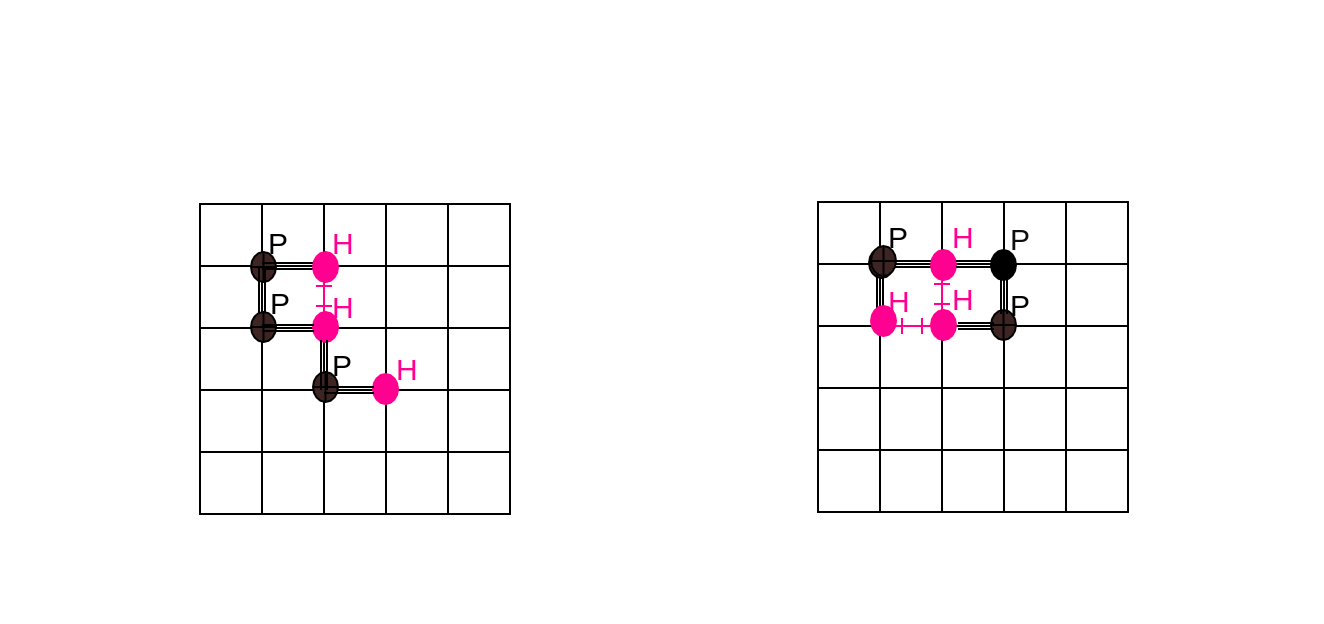
\includegraphics[width=0.9\textwidth]{diagram.png}
    \caption{Przykład włożenia sekwencji $s={HPPHPH}$ w kratę płaską. Po lewej stronie energia całkowita jest równa -1, a po prawej stronie energia całkowita jest równa -2. Co więcej okazuje się, że jest to optymalne globalne rozwiązanie. }
\end{figure}

W tradycyjnym modelu pary $H$-ów z sekwencji $s$ nie są liczone jako formująca wiązanie. Dla uproszczenia, możemy dodać pary $H$-ów w liczeniu energii. Konwencja nie zależy w żaden sposób nie wpływa przy ustalonej sekwencji na minimalizacje energii. 
\mtyt{Trudność tego modelu}


Warto się zastanowić dlaczego ten problem jest ciężki obliczeniowo. Intuicyjnie wydaje się, ze mamy kombinatoryczną własność generowania tras losowych spacerów. Jednak widać, że takich tras jest stosunkowo dużo. \marg{} \marg{Więcej jak estymować ilość takich tras jest w artykule: \href{http://www.deltami.edu.pl/temat/matematyka/zastosowania/2015/04/19/Monte_Carlo_spacery_i_polimery/}{Monte Carlo, Spacery I Polimery prof. Niemiro}} 

Wyżej opisany problem jest problemem obliczeniowych - szukamy minimum funkcji energii. Zastanowimy się, czy potrafimy przeformułować to w problem decyzyjny. Podajmy jego ścisłe sformułowanie.

\textbf{Problem zawinięcia sekwencji}

\newline Wejście: Ustalona sekwencja $s \in \{H,P\}^{n}$, liczbę naturalna $m \in \mathbb{N}$ i kratę $L=\mathbb{Z}^3$. 

\textbf{Pytanie} Czy istnieje zawinięcie sekwencji $s \in \{H,P\}^{n}$ w kracie $
\mathbb{Z}^3$, gdzie ilość połączeń $H \edge H$ jest przynajmniej $m$? 

Istotne jest tutaj określenie trudności tego modelu, czyli potwierdzenie intuicji, że nie umiemy znaleźć szybkiego deterministycznego rozwiązania. Naszym celem będzie prześledzenie rozumowania z tym związanego. 


\todo{zastanów jak podkreslić się tych sąsiadująych}
Zauważmy, ze algorytm rozwiązujący problem zawinięcia sekwencji może zostać wykorzystany w problem poszukiwania minimalnej energii z równania \ref{eq:mai}. Mając algorytm rozwiązujący problem zawijania sekwencji możemy uruchomić go skończenie wiele razy, by uzyskać informacje o minimalnej energii. Dochodzimy do momentu, kiedy algorytm odpowiada nam przecząco, że sekwencja nie istnieje i wtedy kończymy wykonywanie się programu.  

Po chwili dłuższego namysłu okaże się, że nie jest to w cale prosty problem. Nie ma efektywnego algorytmu \marg{Działający w czasie wielomianowym względem długości sekwencji}. 
Rozważając to pytanie ciężko stwierdzić w jaki sposób dobrać algorytm, aby umiał odpowiedzieć prosto na zadane pytanie. Oczywiście można przetestować bardzo brutalnie wszystkie konfiguracje. Jednak dla stosunkowo małych rozmiarów sekwencji problem staje się obliczeniowo niemożliwy do rozwiązania. 


\textbf{Problem perfekcyjnego zawinięcia}
\newline
Wejście: Mając daną sekwencje $s \in \{H,P\}^{n}$ oraz liczbę naturalną $m$ i kratę $L=\mathbb{Z}^3$. 
\newline
Pytanie: Czy istnieje takie zwinięcie $s \in \{H,P\}^{n}$ w $\mathbb{Z}^3$ dla którego połączenia $H \edge H$ są idealnie wpasowane w kostkę rozmiaru $n \times n \times n$. 

\textbf{Przykład}


\todo{obrazek kostki i dopasowania}

W pierwszym kroku do pokazania, że tan problem zawijania sekwencji nie jest łatwy do zawinięcia, pokazuje się że problem perfekcyjnego zawinięcia jest specjalnym przypadkiem problemu zawinięcia sekwencji. Prześledzimy teraz intuicję stojącą za ową redukcją. 

\textbf{Fakt} \newline 
Załóżmy że w naszej sekwencji $s \in \{H,P\}^{n}$ jest $n^{3}$ elementów $H$. Sąsiadujące miejsca sekwencji nie muszą odpowiadać sąsiadującym węzłom w kracie. Wtedy optymalna konfiguracja $S$ w G jest unikalnie osiągnięta poprzez zapakowanie H-ów w $n\times n \times n$ kostce.

Krótki szkic rozumowania:
Każdy z $n^{3}$ w $H$ z sekwencji $s$ ma 6 sąsiadów. Kiedy pakujemy H w $n\times n \times n$ kostce to wszystkie $6n^2$ sąsiadów dla każdego $H'sa$ są również $H$. To jest ponieważ mamy dwa potencjalnie wiązania H-H. 



Teraz najważniejsza cześć, przed nami wprowadzę problem pakowania, który okaże się, że jest bardzo bliski problemowi perfekcyjnego zawinięcia, problem pakowania jest problemem trudnym. 
Co do wniosku pokaże jak wykorzystać ten problem do pokazania trudności problemu zawinięcia sekwencji

\textit{Pytanie}


\textbf{Problem pakowania}
Wejście, mamy skończony zbiór elementów należących do $U$, i funkcje przypisującą rozmiar każdemu elementowi $u \in U$ pozytywną liczbę całkowitą reprezentująca ładowność $B$ i pozytywną liczbę $K$. 
\newline 
\textbf{Pytanie}
Czy jest podział zbioru $U$ na rozłączne zbiory $U_1, \ldots, U_K$ takie, że suma rozmiarów zbiorów jest równa $B$ lub mniejsza. 

Na pierwszy rzut oka nie widać, dlaczego problem pakowania jest bliski problemowi perfekcyjnego zawinięcia. Idea redukcji jednego problemu w drugi opera się na tym, że potrafimy skonsturować pożadany ciąg  



\todo{paradoks i liniowy algorytm}

\marg{ 
}

\end{document}
